\capitulo{1}{Introducción}

Una de las caraterísticas del hombre es su capacidad para el desempeño de tareas complejas. Para llegar a desarrollarlas los individuos tienen que pasar en la mayoría de las ocasiones por un proceso de formación y adiestramiento, pues la simple observación, la intuición, la imitación, etc, por sí solas no suelen lograr que se alcance objetivo o nivel pretendido de conocimientos, habilidades y desempeño. Por esta razón, en todas las sociedades humanas evolucionadas la formación se contempla como uno de sus cimientos más importantes.

Los elementos básicos que componen el proceso de formación-aprendizaje son bien conocidos: el alumno, el profesor, el método de enseñanza y la evaluación. Existen además otros factores como los soportes y sistemas que constituyen el entorno de proceso: el lugar, la forma de trasmistir presencial, a distancia, telemática, en directo, en diferido, con apoyos gráficos, textuales, experimentales, etc.
Este proyecto se ha enfocado en la evaluación de la enseñanza de la programación informática para alumnos principiantes. La corrección de ejercicios de programación puede suponer un trabajo lento y tedioso, que resta tiempo al profesor en su tarea de enseñanza y que puede demorar que el alumno conozca cuál es el resultado de los ejercicios realizados. En definitiva, es un sistema costoso.

Con un diseño adecuado de ejercicios y pruebas sobre los mismos se puede conseguir implementar una corrección automatizada (y rápida) de las respuestas de los alumnos. Éstos además, usando las pruebas proporcionadas por el profesor, pueden ir modificando sus respuestas antes de realizar la entrega final de sus ejercicios. Todo ello redunda en beneficios en el proceso de enseñanaza-aprendizaje: el alumno puede ir comprobando si ha diseñado o no un código que da el resultado esperado, el profesor tiene más tiempo para dedicar a la enseñanza y, se reduce el coste de evaluación.

El presente proyecto desarrolla una plataforma online que se enmarca en el anterior contexto. Permite al profesor poner a disposición de los estudiantes tanto los contenidos de los temas a tratar como tareas que los estudiantes han de resolver relacionadas con tales contenidos. Estos, cuando completan los ejercicios de programación propuestos, los entregan a través de la plataforma y obtienen automáticamente los resultados a la evaluación de sus respuestas.

\begin{figure}[h]
    \centering
    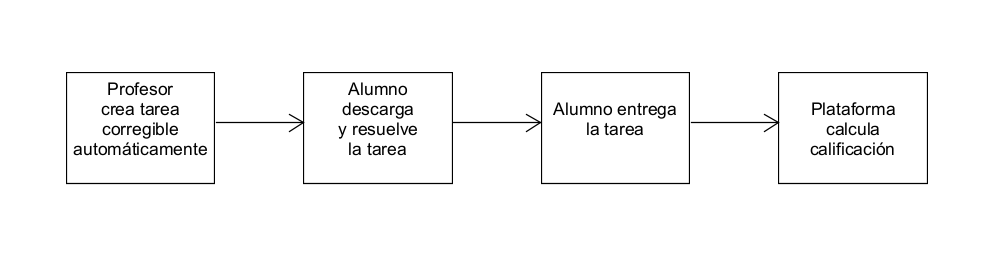
\includegraphics[width=\textwidth]{img/imgs-memoria/FuncionamientoBase.PNG}
    \caption{Funcionamiento Base}
\end{figure}